%%%%%%%%%%%%%%%%%%%%%%%%%%%%%%%%%%%%%%%%%%%%%%%%%%%
% DOCUMENT CLASS DECLARATION
%%%%%%%%%%%%%%%%%%%%%%%%%%%%%%%%%%%%%%%%%%%%%%%%%%%
%% Use the following options:
% \documentclass[paper type% ("letterpaper" required)
% , one or two sided% ("oneside" or "twoside")%
% , font size% ("12pt" required)%
% , document type% ("these", "memoire", "memoirepararticles", "memoireprojet" or "thesepararticles")%
% , document language ("francais" or "english)%
% , addition options% ("creativecommons" if the document is under the creative commons license, "hyperref", "withAlgo2e" to use algorithm2e package with proper formating)
%]{thETS}

%% Exemple with a Ph.D thesis under creative commons, using hyperref
\documentclass[letterpaper%
, twoside%
, 12pt%
,thesepararticles%
, english%
,creativecommons,hyperref, withAlgo2e%
]{thETS}

%%%%%%%%%%%%%%%%%%%%%%%%%%%%%%%%%%%%%%%%%%%%%%%%%%%
% IMPORTANT: PRINTING WITH THE PROPER MARGINS
%%%%%%%%%%%%%%%%%%%%%%%%%%%%%%%%%%%%%%%%%%%%%%%%%%%
%% Always set the "scaling" option to "none" in the prining options 
%% to print the generated PDF with the proper margins.
%%%%%%%%%%%%%%%%%%%%%%%%%%%%%%%%%%%%%%%%%%%%%%%%%%%


%%%%%%%%%%%%%%%%%%%%%%%%%%%%%%%%%%%%%%%%%%%%%%%%%%%
% DECLARATION OF AN ADDITION LIST OF REFERENCES
%%%%%%%%%%%%%%%%%%%%%%%%%%%%%%%%%%%%%%%%%%%%%%%%%%%
%% Exemple of an additional list of references called "refs"
% "refs" is used as a suffix to all bibliography related commands
\newcites{refs}{LIST OF REFERENCES}

%%%%%%%%%%%%%%%%%%%%%%%%%%%%%%%%%%%%%%%%%%%%%%%%%%%
% TITLE PAGE OPTIONS
%%%%%%%%%%%%%%%%%%%%%%%%%%%%%%%%%%%%%%%%%%%%%%%%%%%

\title{Adaptive Collaborative  Autonomous Wireless Networks}

\author{Aytac OZKAN}
\authorcopyright{Aytac Ozkan}

\datesoutenance{"Defense date"}

\datedepot{"Deposit Date"}

\directeur{Prof. Dr.}{Kim Khoa Nguyen}{Department of Electrical Engineering and University of Quebec}

%\directeur{Mrs.}{Prénom Nom}{Nom du département et institution}

\codirecteur{M.}{Pr. Louis Rivest}{PhD Program's Director}

%\codirecteurB{M.}{Prénom Nom}{département et institution}

\president{M.}{First Name Last Name}{Department and institution}

\examinexterne{M.}{First Name Last Name}{Department and institution}

%\jury{Mme.}{Prénom Nom}{département et institution}{}

%%%%%%%%%%%%%%%%%%%%%%%%%%%%%%%%%%%%%%%%%%%%%%%%%%%
% CHANGING THE NAME OF THE DIPLOMA
%%%%%%%%%%%%%%%%%%%%%%%%%%%%%%%%%%%%%%%%%%%%%%%%%%%
%% It is possible to change the name of the diploma to append the concentration by defining \concentration
%\newcommand{\concentration}{ELECTRICAL ENGINEERING}

\listfiles

%%%%%%%%%%%%%%%%%%%%%%%%%%%%%%%%%%%%%%%%%%%%%%%%%%%
% ACTUAL DOCUMENT
%%%%%%%%%%%%%%%%%%%%%%%%%%%%%%%%%%%%%%%%%%%%%%%%%%%
\begin{document}

\pagenumbering{Roman}

%%- Title page -%%
\maketitle

%%- Jury presentation -%%
\presentjury

%%- Foreword -%%
\begin{foreword}

\lipsum[1] % Texte de remplissage pour donner un exemple de la mise en page

\end{foreword}



%%- Acknowledgements -%%
\begin{acknowledgements}

\lipsum[1] % Text filling, to have an example of the layout


\end{acknowledgements}


%%- Summary -%%

\begin{summary}{French title}{mot-clé1, mot-clé2}

\lipsum[1] % Text filling, to have an example of the layout

\end{summary}


%%- Abstract -%%
\begin{abstract}{reinforcement-Learning, transfer-learning,wireless-networks,anti-jamming,multi-agent, collaborative-learning}

Due to the tremendous improvements of technology, the world is more connected than ever to the human history. Mobile devices, cell phones, smart home solutions, autonomous cars, etc. These vehicles are usually using IEEE 802.15.4 communication protocols, the devices which uses this protocol have the limited number of communication channels and low transmit power, are especially susceptible to jamming attacks. For example, some Internet of things (IoT) devices (e.g., brain and heart inculcated IoT devices), jamming attacks can cause serious consequences for human health

Within this concern, to prevent this kind of intentional interference against wireless networks, we are going to employ self-learning algorithms such as deep reinforcement learning to develop a resilient, intelligent, and self-supervised anti-jamming framework.

 Since The DeepMind has been introduced the Reinforcement Learning (RL) and Q-Learning algorithm \cite{ACM:HasseltetSilver}, this tools become one of the major toolkit to develop mitigation and intelligent deceptions strategies to prevent against reactive jamming attacks. Despite it is a subset of machine learning \cite{Kasturi2020MachineLR},it is no need for long training times and large datasets, and this future is the key of its success at the field. 

\end{abstract}


%%- Table of contents -%%
\tableofcontents


%%- List of tables -%%
\listoftables


%%- List of figures -%%
\listoffigures

\listofalgorithms


%%- List of abbreviations -%%
\begin{listofabbr}[3cm]
\item [ETS] École de Technologie Supérieure
\item [ASC] Agence Spatiale Canadienne
\end{listofabbr}


%%- List of symbols -%%
\begin{listofsymbols}[3cm]
\item [a] Première lettre de l'alphabet
\item [A] Première lettre de l'alphabet en majuscule
\end{listofsymbols}


\cleardoublepage

\pagenumbering{arabic}

% Marginpar to the left of the document
\reversemarginpar

%%%%%%%%%%%%%%%%%%%%%%%%%%%%%%%%%%%%%%%%%%%%%%%%%%%
% THESIS EXAMPLE
%%%%%%%%%%%%%%%%%%%%%%%%%%%%%%%%%%%%%%%%%%%%%%%%%%%

\begin{introduction}

The last decade has witnessed the rapid growth of Machine Learning (ML) applications in wireless networks thanks to its agility and efficacy, especially in dealing with uncertainty and dynamics in large-scale problems
    \cite{8743390} \cite{6336689}
However, some recent studies have revealed that conventional ML solutions have shortcomings, especially when they are applied to solve emerging problems in wireless networks, due to the special characteristics of wireless communications, such as high mobility, dynamic environments, diverse connections, and interference. However, some recent studies have revealed that conventional ML solutions have shortcomings, especially when they are applied to solve emerging problems in wireless networks, due to the special characteristics of wireless communications, such as high mobility, dynamic environments, diverse connections, and interference.

Moreover, the performances of ML techniques mainly rely on the availability of training data, but acquiring a sufficient amount of data might be costly and time-consuming. Even if the training data are sufficient, conventional ML techniques usually require a long training time, which makes them impractical for many latency-sensitive applications. Apart from the training time issues, many wire- less devices, e.g., IoT devices, are constrained by their limited computing capacity, and thus they are unable to run high-complexity ML tasks. Moreover, many ML techniques actually create more wireless traffic demands because data have to be sent to a central node for training and processing. Besides causing higher communication overhead, sending raw data may also threaten network users' privacy because sensitive information, e.g., healthcare, is sent via the wireless networks.

To address these challenges, Transfer Learning (TL) has recently emerged as a highly effective solution. Unlike conventional ML techniques that are trained to solve a specific problem, TL leverages valuable knowledge from similar tasks and previous experiences to significantly enhance the learning performance of conventional ML techniques. As a result, TL possesses various advantages over traditional ML approaches, which can be summarized as follows;
\begin{itemize}
	\item Enhance the quality and quantity of training data: One of the most challenging tasks for conventional ML approaches is finding sufficient and high-quality data for the training process. TL can easily overcome this problem by selecting and transferring knowledge from similar domains with a large amount of high-quality data. As a result, TL has been considered a highly effective solution for ML-based wireless networks in the future.
	\item Speed-up learning processes: Instead of learning from scratch like conventional ML approaches, the training process in TL can be significantly sped up thanks to valuable knowledge shared from other similar domains and/or learned in the past. As a result, this can remarkably improve the learning rate, which is especially crucial for the development of ultra-low latency applications for future wireless networks.
	\item Reduce computing demand: Conventional ML approaches usually require a large amount of computing resources for the training processes. However, with TL, most of the data were trained by other source domains before the trained models are transferred to the target do- main, thereby significantly reducing the computing demands for the training process at the target domain. This is particularly useful for wireless devices (e.g., smartphones and edge devices) as they usually have hardware constraints.
	\item Mitigate communication overhead: For TL approaches, instead of sending the raw data with large size, only knowledge, e.g., the weights of trained models, needs to be sent. As a result, the communication overhead can be significantly reduced for wireless networks.
	\item{Protect data privacy: In TL, instead of learning from raw data from other domains, ones only need to learn from their trained models (expressed through weights), and thus data privacy can be protected. This feature of TL is very helpful for privacy-sensitive wireless applications such as healthcare and military communication networks.}
\end{itemize}

\end{introduction}

%%- Uncomment the literature review for a thesis by articles -%%
%\begin{literaturereview}

%\end{literaturereview}

%%- First demo chapter -%%
\chapter{Research Objectives, Motivation, Research Questions}

\section{Research Objectives}

The main purpose of this research is to develop efficient, reliable, and relentless mitigation techniques against the jammer, particularly reactive and powerful ones by employing machine learning (ML) and wireless communication technologies. 

To achieve the objective defined above, we are going to use the Frequency Hopping Spectrum  Sensing (FHSS) technique. In the infinite time space, regarding the probability distribution of incoming signals, we are going to build the most accurate ML model to find out  the optimal and feasible prediction for communication channels.

Of course, the first paragraph is specified only the core part of the communication node, but the particular contribution of this research is to develop multi-agent (multi-node) collaborative (transfer meta-learning) learning techniques to satisfy the constraints such as cost of learning (for each node), cost of transferring mitigation strategy. Predicate on these details, we would like to acquire an augmented Markov decision tuple for our ML model.

Therefore, we can divide our main objective into three subsections and each of them address a different research problem.

We assume in the wireless ad-hoc network, there are two communication node (CN) and one reactive jammer. Also CN1 and CN2 has data connection, which means they can transmit the data to each other. In addition, the ad-hoc network is multi-channel. Constraints, respectively CN's power storage (limit), channel bandwidth, and installed CPU or GPU power on the CN. 

\subsection{Objectives}

\begin{itemize}
 \item {In the infinite time space, we are going to build a Machine Learning model which will take as input frequencies by sensing from the wireless network, and try to predict the jammer next action (channel estimation), which literally means that try to determine the next communication channel will jam. And it will allow us to determine the jamming activity pattern in the ad-hoc network, and by analyzing these patterns we are going to concrete  mitigation strategies. So, related research will propose novel techniques to answer the question below,
     
     How to catalyze the jamming activity pattern and initialize effective and relentless mitigation strategies for communication nodes in wireless ad-hoc networks by using autonomous learning techniques ?}
 \item {In the first item, we have proposed a method which allows us to analyze the jammer behaviour pattern, and generate defence strategies for the CN based on this pattern. However, in the wireless spectrum we have two different CNs and we can have more nodes, in this case we may transfer the produced policy (or strategy) from one node to another when suitable conditions are satisfied. Moreover, collaborative learning can increase the chances to mitigate against reactive and strong jammers by saving time and energy of CNs. E.g, the cost of learning, cost of transmission, and accuracy of learning models have  high importance roles in the decision model of the framework. 
  
 	Therefore, related research will address the question below, 
 	How the collaborative (transfer) learning can assist knowledge transmission between two different communication nodes in the wireless ad-hoc communication spectrum ? 
 }

 \item{In second item we introduced collective (transfer learning) technique, but when a jamming attack hit the wireless network, there won't be any data transmission in this condition, each CNs have to run their own learning algorithm. } 
 
\end{itemize}

%%- Second demo chapter -%%
\chapter{Literature Review}


\chapter{Proposed methodologies}

\section{Preliminaries}


\subsection{Fundamentals of Transfer Learning}


Transfer Learning, simply learned knowledge will be transferred from the source domain to the target domain to improve the learning process of the target task. Thus, in the following, we first present the definition of a "domain" and  In our research problem, the source domain is the communication node (CN) that underwent the jammer attack, And the target domain is the likelihood closest unattacked communication node in the wireless network.

\begin{definition}
''Domain: A domain $\displaystyle \mathcal{D}$ is defined by two parts: (i) a feature space $\displaystyle \mathcal{X}$ and (ii) a marginal probability distribution $\displaystyle \mathcal{P}( X)$ in which $\displaystyle X\ =\ \{x_{1,\dotsc ,x_{n}}\} \ \in \ \mathcal{X}$ where $\displaystyle n$ is the number of feature vectors in $\displaystyle \mathcal{X} .$ As such $\displaystyle \mathcal{D} \ =\ \{\mathcal{X} ,\mathcal{P}( X)\}$."
\end{definition}

\begin{definition}
"Task: given domain $\displaystyle \mathcal{D}$, a task $\displaystyle \mathcal{T}$ is defined by two parts: (i) a label space $\displaystyle \mathcal{L}$ and (ii) a predictive function $\displaystyle f( .)$. The predictive function (or decision function) is learned from the feature vector and label space pairs $\displaystyle \{x_{i,\ l_{i}}\}$, with \ $\displaystyle x_{i} \ \in \ X$ and $\displaystyle l_{i} \ \in \ \mathcal{L}$. In other words, a task is defined by $\displaystyle \mathcal{T} \ =\ \{\mathcal{L} ,\ f( .)\}$."
\end{definition}

\begin{definition}
"Transfer Learning: Given a source domain $\displaystyle \mathcal{D}_{S}$ with a corresponding source task \ $\displaystyle \mathcal{T}_{S}$ and a target domain $\displaystyle \mathcal{D}_{T}$ with a corresponding target task $\displaystyle \mathcal{T}_{T}$, the goal of TL is to learn the target predictive function $\displaystyle f_{T}( .)$ by leveraging the knowledge gained from $\displaystyle \mathcal{D}_{S}$ and $\displaystyle \mathcal{T}_{S}$ where $\displaystyle \mathcal{D}_{S} \ \neq \ \mathcal{D}_{T}$ or $\displaystyle \mathcal{T}_{S} \ \neq \ \mathcal{T}_{T}$."
\end{definition}



\section{Problem Statement}

\begin{table}[!h]
        \centering        
\begin{tabular}{|p{0.50\textwidth}|p{0.50\textwidth}|}
\hline 
 Notation & Description \\
\hline 
 $\displaystyle P_{s}( k)$ & Transmit power of the sender  \\
\hline 
 $\displaystyle P^{l}_{J}( k)$ & Jamming power of the $\displaystyle lth$ jammer \\
\hline 
 R & number of \ transmit power levels \\
\hline 
 I & number of jamming power levels \\
\hline 
 L & number of jammers \\
\hline 
 N  & number of channels \\
\hline 
 $\displaystyle x^{( k)}$ & channel chosen by the sender \\
\hline 
 $\displaystyle y^{( k)}_{l}$ & channel choosen by the $\displaystyle lth$ jammer \\
\hline 
 $\displaystyle h_{s}$ & channel power gain of the sender \\
\hline 
 $\displaystyle h_{l}$ & channel power gain of the $\displaystyle lth\ $ jammer \\
 \hline
\end{tabular}        
\end{table}

We consider a wireless communication scenario where a sender such as a wireless device \ transmits \ data to the receiver at time slot $\displaystyle k$ with a transmit power $\displaystyle P_{s}( k)$. while there are L Jammers who can launch jamming attacks by injecting meaningless interference signals denoted as $\displaystyle P^{l}_{j}( k) \ \in \ \left\{P^{1}_{j}( k) ,P^{2}_{j}( k) ,...,P^{L}_{j}( k)\right\} .$

Each $\displaystyle P^{l}_{j}( k)$ has $\displaystyle I$ different power levels. 

In our model, each jammer is assumed to attack only one channel, At time slot $\displaystyle k,$the sender can choose one of N selectable frequency channels for transmitting denoted by $\displaystyle x^{( k)} .$ Meanwhile, $\displaystyle L$ jammers may select their frequency channels (denoted as $\displaystyle \left\{y^{( k)}_{1} ,\ y^{( k)}_{2} ,\dotsc ,y^{( k)}_{L}\right\}$) for jamming. 

$\displaystyle h_{s}$ and $\displaystyle h_{l}$ denote the channel power gains from the sender and the $\displaystyle lth$ jammer to the receiver respectively. 

To resist the jamming attack, the sender needs to choose an unblocked channel $\displaystyle x^{( k)}$ and an appropriate transmit power. In general, variable transmit power model is shown to be superior to the constant transmit power one under the constraint of the same average power. \ After the receiver gets the signal at time slot k, the $\displaystyle SINR( k)$ is calculated by (1) and returned to the sender through the feedback channel. 

\begin{equation}
SINR( k) \ =\ \frac{P_{s}( k) h_{s}}{\beta +\sum ^{L}_{l=1} P^{l}_{J}( k) h_{l} f\left( x^{( k)} \ =\ y^{( k)}_{l}\right)},
\end{equation}

 where $\displaystyle \beta $ is the receiver noise power, $\displaystyle P^{l}_{J}( k)$ denotes the jamming power chosen by the $\displaystyle lth$ jammer and $\displaystyle f( \xi )$ is an indicator function that equals 1 if $\displaystyle \xi $ is true and 0 otherwise. If the jammer is completely blocked by the jammer at time slot k, the sender needs to retransmit the signal \ This will consume extra energy denoted as $\displaystyle C_{m} .$

It is reasonable that the channel is considered blocked if the jamming power takes the maximum value $\displaystyle P^{L}_{J}( k) .$ In order to make a tradeoff between the energy saving and the communication performance, we define the utility $\displaystyle u^{( k)}_{s}$ of the sender by: 

\begin{equation}
u^{( k)}_{s} \ =\ SINR( k) \ -\ C_{m} f\left( P^{I}_{J}( k) \ =\ P^{L}_{j}( k)\right) f\left( x^{( k)} \ =\ y^{( k)}_{l}\right) \ -\ \frac{C_{s} P_{s}( k)}{P^{max}_{s}}
\end{equation}

where $\displaystyle C_{S}$ and $\displaystyle P^{\max}_{S}$ denote the unit transmission cost and the maximum transmit power, respectively. 

\begin{algorithm}[!h]

\caption{Algorithm example}

\KwIn{Gallery with initial templates $\mathcal G = \{\textbf{r}_1,...,\textbf{r}_J\}$, unlabeled adaptation set $\mathcal D = \{\textbf{d}_{1},...,\textbf{d}_{L}\}$}
\KwOut{Updated Gallery $\mathcal G' = \{\textbf{r}_1,...,\textbf{r}_{J'}\}$, $J' \geq J$}
\BlankLine
\BlankLine

Estimate updating threshold $\gamma^u \geq \gamma^d$ from $\mathcal G$\;

$\mathcal G \leftarrow \mathcal G'$\tcc*{update gallery}

	\For{all samples $d_l \in \mathcal D$ ($l=1,...,L$)}{
		\For{all references $r_j \in \mathcal G$ ($j=1,...,J$)}{
			$s_j(\textbf{d}_l) \leftarrow similarity\_measure(\textbf{d}_l,\textbf{r}_j)$\;
		}
	}
	
	$S(\textbf{d}_l) \leftarrow \max\limits_{j \in [1,J]}\{s_j(\textbf{d}_l)\}$\;
	
	\If{$S(\textbf{d}_l) \geq \gamma_d$}{
		Output positive prediction\;
		
		\If{$S(\textbf{d}_l)\geq \gamma^u$}{
			$\mathcal{G'} \leftarrow \mathcal{G'} \cup \textbf{d}_l$\;
		}
		
	}
\end{algorithm}


\chapter{Preliminary Results}


%%- Conclusion -%%
\begin{conclusion}

\lipsum[1] % Text filling, to have an example of the layout

\end{conclusion}


%%%%%%%%%%%%%%%%%%%%%%%%%%%%%%%%%%%%%%%%%%%%%%%%%%%
%  Appendix example:
%%%%%%%%%%%%%%%%%%%%%%%%%%%%%%%%%%%%%%%%%%%%%%%%%%%
\appendix

%% To use more than one appendix
\multiannexe

%% Appendix from an external file
% \include{extApp}

\chapter{Appendix example}


\section{First section of the appendix}


\subsection{Figures in annexes}

\begin{figure}
	\centering
	\fbox{
		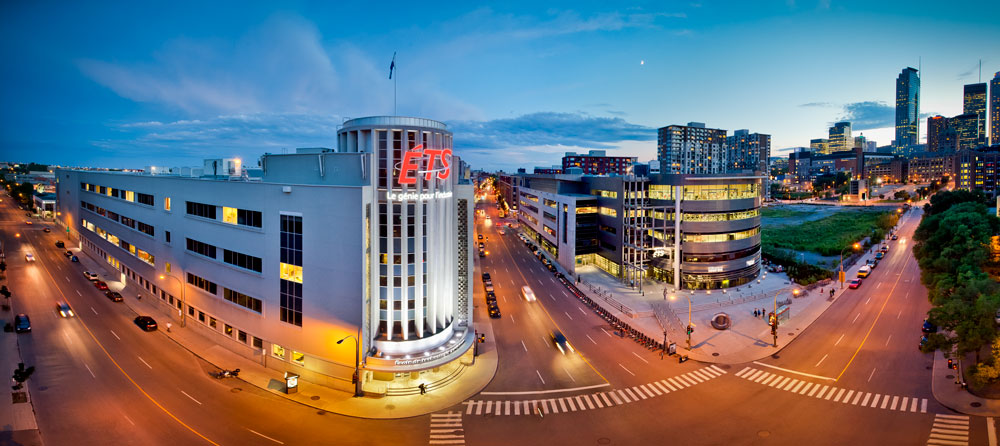
\includegraphics[width=0.75\textwidth]{Figures/vueEts.jpg}
	}
	 \\ \parbox{0.7\textwidth}{\caption{Figure in an appendix}\label{fig:testAp}}
\end{figure}

\begin{figure}
	\centering
	\fbox{
	\parbox{0.975\linewidth}{
	\subfloat[first figure]{
		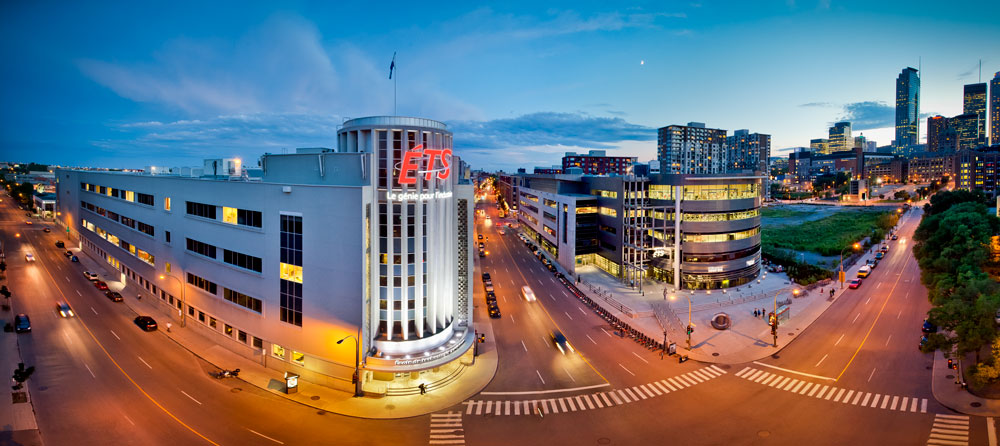
\includegraphics[width=0.47\linewidth]{Figures/vueEts.jpg}
	}\hspace{0.009\linewidth}
	\subfloat[second figure]{
		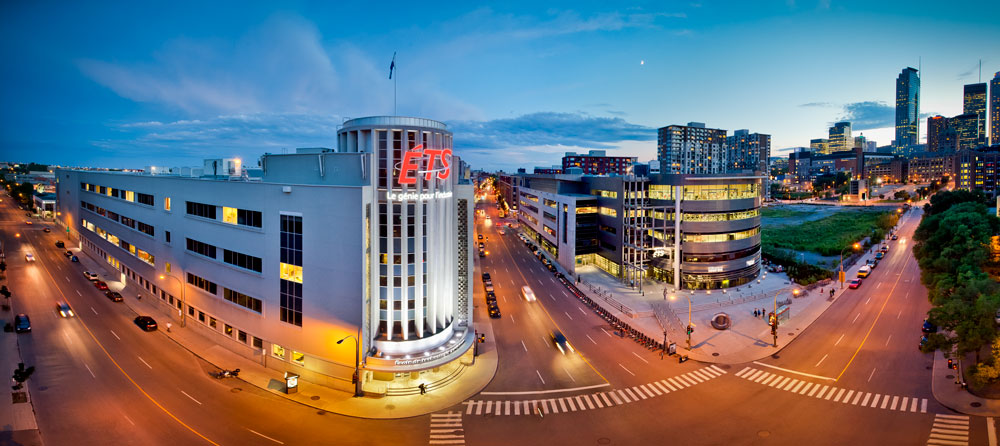
\includegraphics[width=0.47\linewidth]{Figures/vueEts.jpg}
	}
	
	\subfloat[third figure]{
		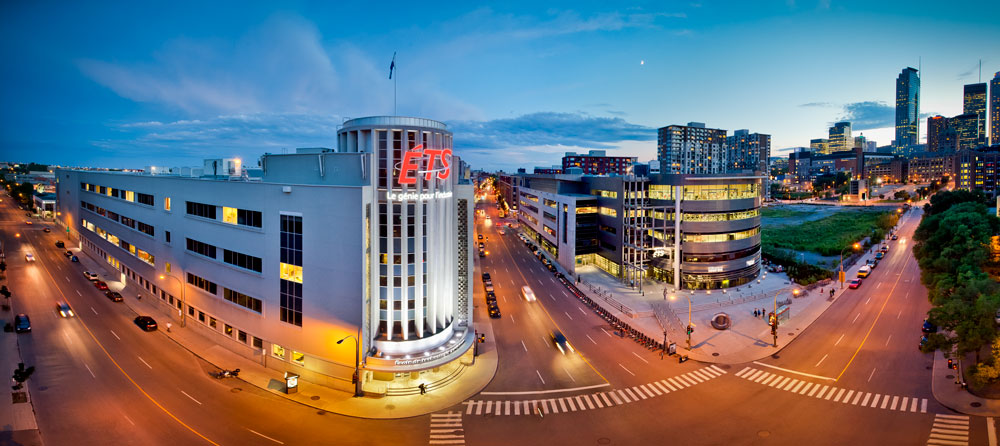
\includegraphics[width=0.47\linewidth]{Figures/vueEts.jpg}
	}\hspace{0.009\linewidth}
	\subfloat[fourth figure]{
		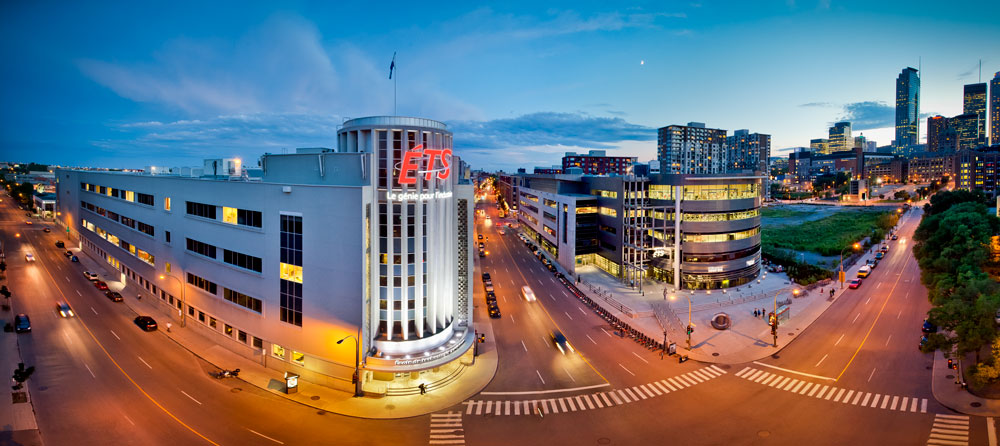
\includegraphics[width=0.47\linewidth]{Figures/vueEts.jpg}
	}}}
	\\ \parbox{0.975\linewidth}{\caption{Subfig example}}
\end{figure}

In the annexes, the figures are declared in the same way. Their numbering changes automatically (e.g. Figure \ref{fig:testAp}).

\subsubsection{Tables in annexes}

\begin{table}
		\parbox{0.65\textwidth}{\caption{Table in an appendix}\label{tab:testAp}}

		\begin{tabular}{|c|c|c|c|c|c|c|c|}
		\hline
			{\bf titre} & {\bf titre} & {\bf titre} & {\bf titre} & {\bf titre} & {\bf titre} & {\bf titre} & {\bf titre} \\
	  \hline
			blá & blá & blá & blá & blá & blá & blá & blá \\
	  \hline
			blá & blá & blá & blá & blá & blá & blá & blá \\
	  \hline
			blá & blá & blá & blá & blá & blá & blá & blá \\
	  \hline
			blá & blá & blá & blá & blá & blá & blá & blá \\
	  \hline
			blá & blá & blá & blá & blá & blá & blá & blá \\
	  \hline
			blá & blá & blá & blá & blá & blá & blá & blá \\
	  \hline
		\end{tabular}
\end{table}

Same behaviour for the tables (e.g., Table \ref{tab:testAp}).


%%%%%%%%%%%%%%%%%%%%%%%%%%%%%%%%%%%%%%%%%%%%%%%%%%%
% BIBLIOGRAPHY AND REFERENCES
%%%%%%%%%%%%%%%%%%%%%%%%%%%%%%%%%%%%%%%%%%%%%%%%%%%

%%- Bibliography -%%
\newpage
% Single spacing for the bibliography
\begin{spacing}{1}
    \setlength{\bibsep}{\baselineskip}
	\nocite{*} % The "nocite" command can be used to print references that haven't been used in the document. The "*" option specifies that every reference should be printed
	\bibliographystyle{bibETS} % ETS bibliography style
	\addcontentsline{toc}{chapter}{BIBLIOGRAPHY} % Addition of the bibliography in the table of contents

	\bibliography{biblio_en} % List of bibliography files, biblio.bib is an example

\end{spacing}

%%- Other list of references, "refs" example --%
%%%%%%%%%%%%%%%%%%%%%%%%%%%%%%%%%%%%%%%%%%%%%%%%%%%
% IMPORTANT: HOW TO COMPILE AND PRINT ADDITIONAL REFERENCES (replace "refs" by the chosen name)
%%%%%%%%%%%%%%%%%%%%%%%%%%%%%%%%%%%%%%%%%%%%%%%%%%%
% Follow these three steps:
%   1. Compile the document once, to save the used references in refs.aux
%   2. Compile the references
% 		- On Linux: Use the "bibtex refs" command in the document folder
%		- On MacOSX (MacTex distribution): Use the "/usr/texbin/bibtex refs" command in the document folder
%		- On Windows: Edit the "update_refs.bat" script to put the right suffix ("refs" here), and launch the script
%   3. Recompile the document TWICE
%%%%%%%%%%%%%%%%%%%%%%%%%%%%%%%%%%%%%%%%%%%%%%%%%%%

\newpage
% Same commands than for the bibliography, only with the "refs" suffix
\begin{spacing}{1}
    \setlength{\bibsep}{\baselineskip}
	%\nociterefs{*}
	\bibliographystylerefs{bibETS}
	\addcontentsline{toc}{chapter}{LIST OF REFERENCES}

	\bibliographyrefs{refs}

\end{spacing}

\end{document}